\section{空气}\label{sec:1-1}

空气是我们经常接触的物质,但是人们研究空气的成分却比较晚。
这因为空气是一种既看不见踪影又闻不着气味的气体。人们曾长期认为空气是一种单一的物质。
后来,人们对燃烧现象和空气组成作了深入的研究,才认识到空气并不是单一的物质。
那么,空气究竟是由哪些物质组成的?

很多有科学家为解决这个问题作了许多研究工作。

早在十八世纪七十年代,瑞典化学家舍勒和英国化学家普利斯特里\footnote{舍勒(Scheele,1742 —\, 1786);普利斯特里(Priestley,1733 一 1804)。}%
曾先后用加热某些物质的不同方法,分别发现并制得了一种气体,它能使物质燃烧得更旺,这就是现在所说的氧气。
但当时流传着一种错误的理论,认为物质能够燃烧,是因为其中含有一种“燃素”的特殊东西,
物质燃烧就是物质失去了这种特殊东西而变成灰烬或残渣。
舍勒和普利斯特里没有摆脱这种当时占统治地位的错误理论的束缚,
未能对燃烧现象作出正确的解释,没有得出燃烧是物质跟空气里含有的氧气起反应的科学结论。

法国化学家拉瓦锡\footnote{拉瓦锡(Lavoisier, 1743 —\, 1794)。}最早运用天平作为研究化学的工具,在实验里重视化学反应中物质质量的变化。
当拉瓦锡知道了普利斯特里制取氧气的方法后,就做了一个著名的实验\footnote{见小号楷体字材料。小号楷体字材料是供学生课外阅读的。}。
他摆脱了传统的错误理论的束缚,尊重事实,对实验作了科学的分析和判断,
揭示了燃烧是物质跟空气里的氧气发生了反应,指出了物质里根本不存在一种所谓燃素的特殊东西。
拉瓦锡在前人工作的基础上,通过实验得出了空气是由氧气和氮气组成的结论。

\begin{yuedu}

\begin{wrapfigure}[10]{r}{7cm}
    \centering
    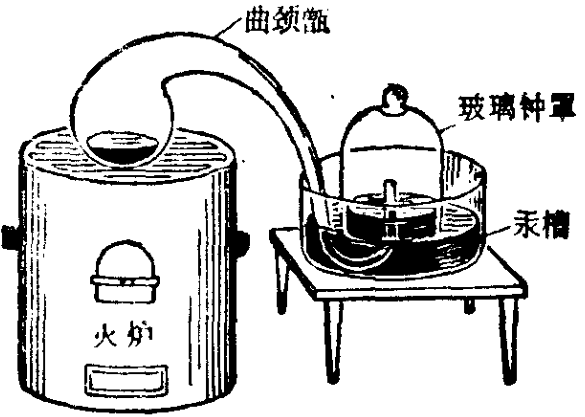
\includegraphics[width=5cm]{../pic/czhx1-ch1-1}
    \caption{拉瓦锡研究空气成分所用的装置}\label{fig:1-1}
\end{wrapfigure}

    拉瓦锡研究空气成分的实验是怎样进行的呢?

    拉瓦锡把少量汞(俗称水银)放在密闭的容器(图 \ref{fig:1-1})里连续加热 $12$ 天。
    结果发现,有一部分银白色的液态汞变成红色粉末,同时容器里的空气的体积差不多减少了 $1/5$。
    拉瓦锡研究了剩余的那部分空气,发现这部分空气既不能供给呼吸,维持动物的生命,也不能支持燃烧。
    它就是我们现在所说的氮气(拉丁文原意是“不能维持生命”)。

    拉瓦锡把汞表面上所生成的红色粉末(后来证明是氧化汞)收集起来,放在另一个较小的容器里再加强热,
    得到了汞和氧气,而且氧气的体积恰好等于密闭容器里所减少的空气的体积。
    他把得到的氧气加到前一个容器里剩下的约 $4/5$ 体积的气体里去,结果得到的气体跟空气的性质完全一样。
    通过这些实脸,拉瓦锡得出了空气是由氧气和氮气组成的结论。

\end{yuedu}


我们可以回忆小学自然常识课里,证明空气里含有氧气和氮气两种成分的实验。

在十九世纪末以前,人们都深信空气里仅含有氧气和氮气两种气体。
空气里是不是只含有氧气和氮气呢?十九世纪末,科学家又做了不少实验,终于发现,空气里还含有
氦、氖、氩、氪、氙\footnote{氦\,音\pinyin{hai4}、氖\,音\pinyin{nai3}、氩\,音\pinyin{ya4}、氪\,音\pinyin{ke4}、氙\,音\pinyin{xian1}}等惰性气体。

此外,空气里还含少量的二氧化碳、水蒸气以及其它气体和杂质。

空气的成分按体积计算,大致是:氧气 $21\%$, 氮气 $78\%$,惰性气体 $0.94\%$,二氧化碳 $0.03\%$,
其它气体和杂质 $0.03\%$(图\ref{fig:1-2})。

\begin{figure}[htbp]
    \centering
    \begin{tikzpicture}
    \draw (0, 0) rectangle (10, 2);
    \draw (7.8, 0) -- (7.8, 2);
    \draw (7.8, 0.2) -- (10, 0.2);
    \draw (9.7, 0) -- (9.7, 0.2);
    \draw [fill=black] (9.7, 0) rectangle (10, 0.1);

    \node at (4, 1) {氮气$78\%$};
    \node at (8.8, 1) {氧气$21\%$};
    \draw (8.2, 0.1) -- (7.8, -0.2) node [left] {惰性气体$0.94\%$};
    \draw (9.85, 0.15) -- (7.8, -0.6) node [left] {二氧化碳$0.03\%$};
    \draw (9.85, 0.05) -- (8.9, -1.0) node [left] {其它气体和杂质$0.03\%$};
\end{tikzpicture}


    \caption{空气的成分(按体积计算)}\label{fig:1-2}
\end{figure}

空气的成分一般说来是比较固定的。但是,自近代以来,随着工业的发展和燃料用量的激增,
排放到空中的一些有害气体和烟尘,改变了空气的成分.并且使空气受到污染。
例如,煤燃烧产生的废气,石油化工厂排放的毒气,汽车排气形成的烟雾,等等,
使一些城市的空气污染日益严重,对人类造成很大的危害。
我们一定要采取各种措施,防止空气受到污染,保护环境,为人类生活提供清洁的空气。

空气是一种十分重要的天然资源。在我们国家里,随着社会主义建设事业的发展,
从空气里分离出来的氧气、氮气和惰性气体,已经广泛地应用在工农业生产和国防建设中。

氧气的性质和用途将在下节介绍。现在我们先简略地认识一下氮气和惰性气体的性质及其用途。

在通常状况\footnote{通常情况一般指的是在 $20$ ℃ 左右和大约 $1$ 标准大气压时的状况。}下,
氮气是没有颜色、没有气味的气体,它很难跟其它物质发生变化。
但是在一定条条件下,氮气也能跟其它物质发生化学反应。
我们常利用氮气的这种性质来制取氮肥、炸药等等。因此,氮气是一种重要的化学工业原料。
氮气对农业生产也很重要,空气里的氮气被豆科作物根瘤菌固定后,能够成为作物的氮素养料。

氦、氖、氩、氪、氙等惰性气体都是没有颜色、没有气味的气体。

\begin{yuedu}

    惰性气体是怎样被发现的呢?

    二百多年前,人们已经知道,空气里除了少量的水蒸气、二氧化碳外,其余的就是氧气和氮气。
    1785 年,英国科学家卡文迪许\footnote{卡文迪许(Cavendish,1731 —\, 1810)。}通过实验发现,
    把不含水蒸气、二氧化碳的空气除去氧气和氮气后,仍有很少量的残余气体存在。这种现象在当时并没有引起化学家的重视。
    一百多年后,英国物理学家雷利\footnote{雷利(Rayleigh,1842 —\, 1919)。} 测定氮气的密度时,
    发观从空气里分离出的氮气每升质量是 $1.2572$ 克,而从含氮物质制得的氮气每升质量是 $1.2505$ 克。
    经多次测定,两者质量相差仍是几毫克。
    可贵的是雷利没有忽视这种微小的差异,他怀疑从空气分离出来的氮气里含有没被发现的较重的气体。
    于是,他查阅了卡文迪许过去写的资料,并重新做了实验。
    1894 年,他在除掉空气里的氧气和氮气以后,得到了很少量的极不活泼的气体。
    与此同雷利的朋友、英国化学家拉姆塞\footnote{拉姆塞(Ramsay,1852 —\, 1916)。}用其它方法从空气里也得到了这样的气体。
    经过分析,判断该气体是一种新物质\footnote{实际上,这一气体里除氩气外仍含有极少量的其它惰性气体。}。
    由于这气体极不活泼,所以命名为氩(拉丁文原意是“懒惰”)。

    以后几年里,拉姆塞等人又陆续从空气里发现氦气、氖气、氪气和氙气。

\end{yuedu}


过去,人们认为氦气、氖气、氩气、氪气、氙气等不跟其它物质发生化学反应,因此把它们叫做惰性气体。
现在,人们通过科学实验已经发现,在一定条件下,有些惰性气体也能跟某些物质发生化学反应,生成其它物质。
因此,我们平常按习惯叫的惰性气体,它们的 “惰性” 是相对的,而不是绝对的。

惰性气体在空气里的含量很少,所以又叫做稀有气体。随着科学技术的发展,惰性气体的应用越来越广泛。

由于惰性气体一般不跟其它物质发生化学反应,人们利用这种性质,在一些工业生产中,常常把它们用作保护气。
例如,用电弧焊接火箭、飞机、轮船、导弹等用的不锈钢、铝或铝合金等时,可以用氩气来隔绝空气,防止金属在高温下跟其它物质起反应。
还可以把氩气和氮气的混和气体充入灯泡里,使灯泡经久耐用。

惰性气体在通电时会发出有色的光。因此,它们在电光源中有特殊的应用。
灯管里充入氩气.通电时会发出紫蓝色光;充入氦气,通电时会发出粉红色光;
充入氖气,通电时会发出红光,这种光能穿透浓雾,所以氖灯可用作航空、航海的指示灯。
五光十色的霓虹灯就是利用惰性气体的这种性质制成的。
在石英玻璃管里充入氙气的氙灯,通电时能发出比萤光灯强几万倍的强光,因此叫做 “人造小太阳” 。
这种灯可用于广场、体育场、飞机场等的照明。

氖气、氪气、氙气还可用于激光技术等方面。
氦气在原子反应堆技术中可用作冷却剂。
作为麻醉剂,氙气在医学上也很受重视。


\begin{xiti}

\xiaoti{填空:}

空气的成分按体积计算,大致是 \xhx 占 $21\%$,\xhx 占 $78\%$,
\xhx 占 $0.94\%$,\xhx 占 $0.03\%$ 以及 \xhx 占 $0.03\%$。所以说,
空气的成分以 \xhx 、\xhx 为主,其中 \xhx 约占空气体积的 $1/5$,
\xhx 约占空气体积的 $4/5$。

\xiaoti{举例说明氮气的主要用途。}

\xiaoti{下列关于惰性气体的叙述,哪个是错误的?把错误的叙述加以改正。}
\begin{xiaoxiaotis}

    \xxt{惰性气体是氦、氖、氩、氪、氙等气体的总称。}

    \xxt{惰性气体不跟其它物质发生化学反应。}

    \xxt{灯管里分别充入氦气、氖气或氩气等惰性气体,通电时会发出不同的有色光。}

\end{xiaoxiaotis}

\end{xiti}


